\documentclass[blue]{beamer}
\usepackage{beamerthemesplit}
\usetheme{Warsaw}
\usepackage[polish]{babel}
\usepackage[utf8]{inputenc}
\usepackage[T1]{fontenc}
\usepackage{amssymb}
%\usepackage{graphicx}
%\usepackage{epstopdf}

\title{PAAL}
\author{Piotr Jaszkowski, Mateusz Machalica, Grzegorz Prusak, Łukasz Solak}
\date{7 czerwca 2013}

\begin{document}
\setbeamercovered{transparent}

\begin{frame}
\titlepage
\end{frame}

\begin{frame}
\begin{block}{Metaheurystyka}
Ogólny algorytm (heurystyka) do rozwiązywania problemów obliczeniowych.
Algorytm metaheurystyczny można używać do rozwiązywania dowolnego problemu,
który można opisać za pomocą pewnych definiowaych przez ten algorytm pojęć. (...)
Określenie powstało z połączenia słowa ''meta'' (''nad'', tutaj w znaczeniu ''wyższego poziomu'')
oraz słowa ''heurystyka'' (gr. heuriskein - szukać), co wynika z faktu, że algorytmy
tego typu nie rozwiązują bezpośrednio żadnego problemu, a jedynie podają sposób na utworzenie odpowiedniego algorytmu.
\footnote{źródło: \url{http://pl.wikipedia.org/wiki/Metaheurystyka}}
\end{block}
\end{frame}

\begin{frame}{Problem minimalizacyjny}
\begin{block}{Problem minimalizacyjny}
definiuje funkcję kosztu na przestrzeni rozwiązań do zminimalizowania.
\end{block}
\begin{figure}
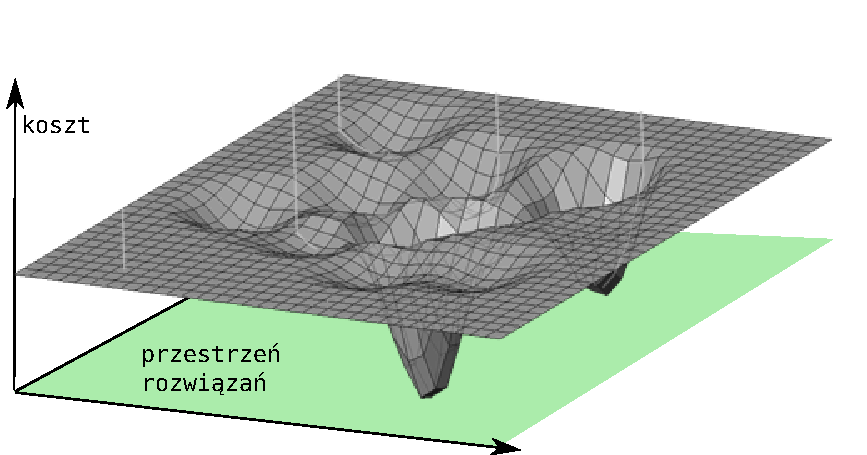
\includegraphics[scale=.7]{ss1.pdf}
\end{figure}
\end{frame}

\begin{frame}{topologia 2-opt dla TSP}
\begin{block}{Sąsiedztwo rozwiązania w 2-opt}
składa się z rozwiązań
powstałych przez odwrócenie spójnego
fragmentu danego rozwiązania.
\end{block}
\begin{figure}
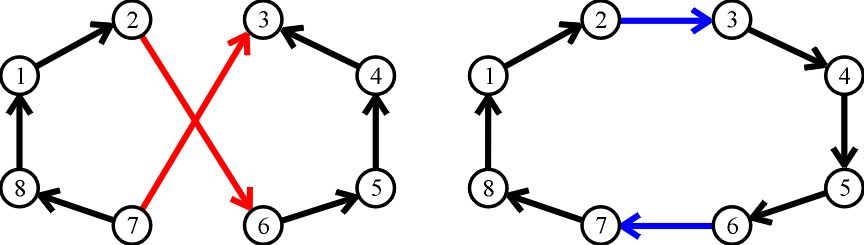
\includegraphics[scale=.7]{2opt.jpg}
\end{figure}
\end{frame}

\begin{frame}{przebieg local search'a}
\begin{figure}
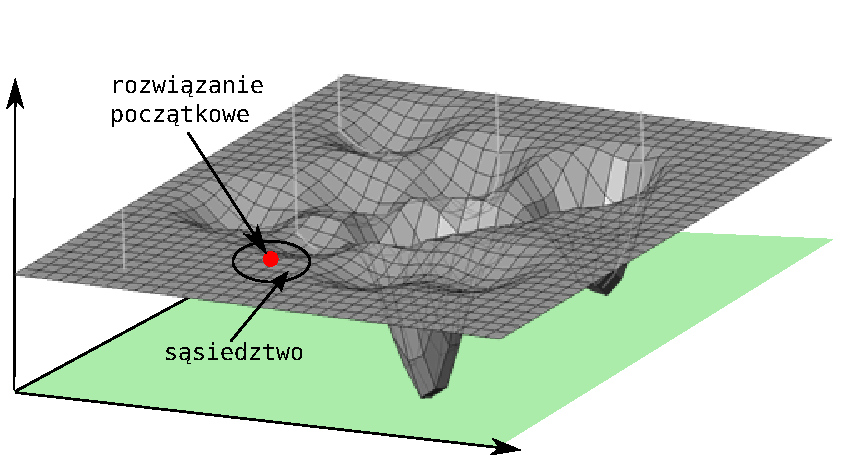
\includegraphics[scale=.7]{ss2.pdf}
\end{figure}
\end{frame}

\begin{frame}{przebieg local search'a}
\begin{figure}
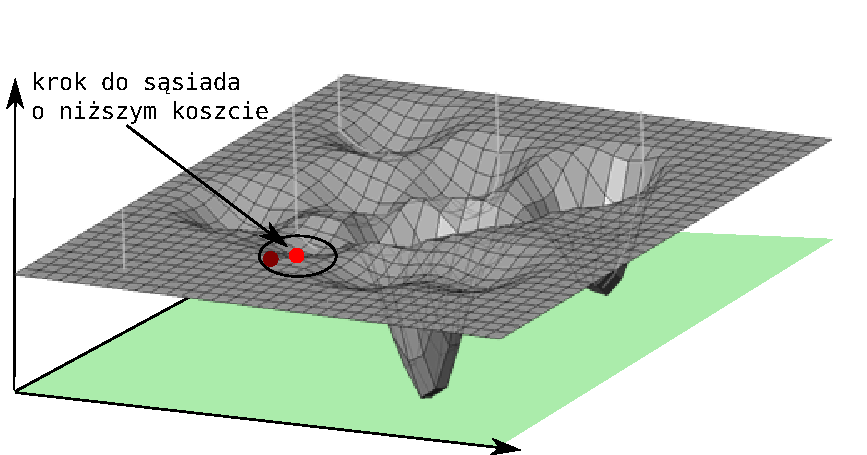
\includegraphics[scale=.7]{ss3.pdf}
\end{figure}
\end{frame}

\begin{frame}{przebieg local search'a}
\begin{figure}
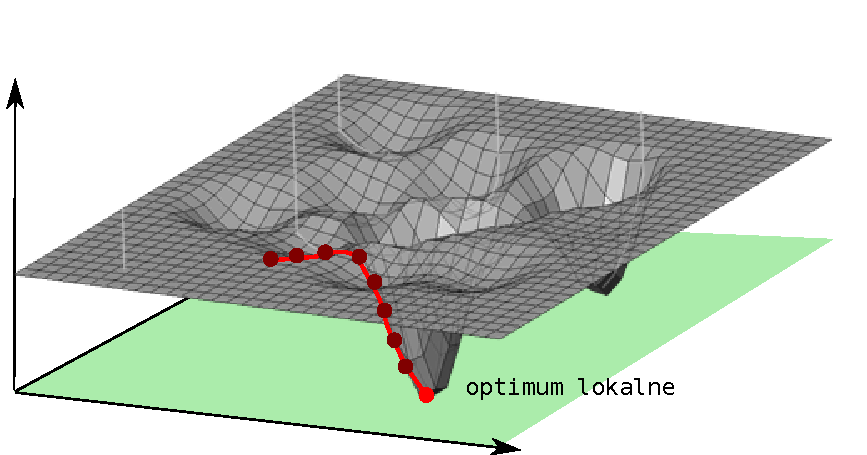
\includegraphics[scale=.7]{ss4.pdf}
\end{figure}
\end{frame}


\end{document}
